\documentclass{article}
\usepackage[UTF8]{ctex}
\usepackage{geometry}
\usepackage{tikz}
\usepackage{float}
\usetikzlibrary{positioning, shapes, arrows.meta, fit, calc, backgrounds, chains}

\geometry{a4paper, margin=1in}

\title{卷积模块设计与分析报告}
\author{CS207 Project Team}
\date{\today}

\begin{document}

\maketitle

\section{系统架构简易框图及卷积模块位置}

本系统采用分层设计,卷积模块 \texttt{matrix\_alu} 位于功能层(Functional Layer)的计算子系统(Calc Sys)中。

\begin{figure}[H]
\centering
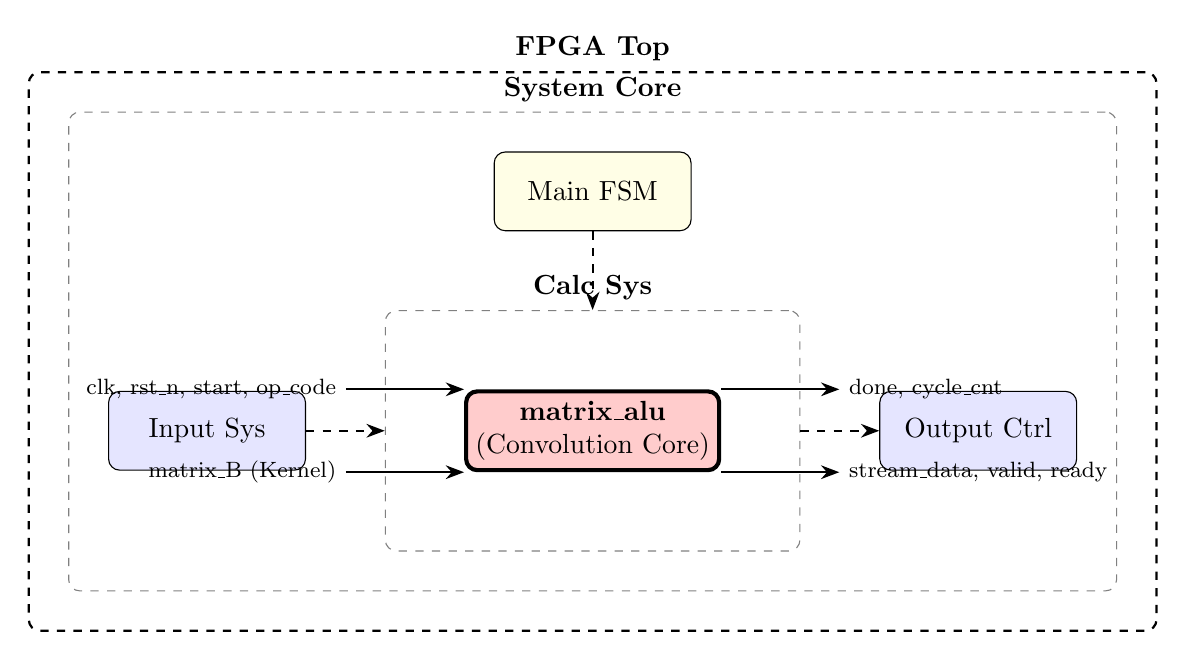
\begin{tikzpicture}[
    node distance=1cm and 1cm,
    box/.style={rectangle, draw=black, rounded corners, minimum width=2.5cm, minimum height=1cm, align=center, fill=white},
    container/.style={rectangle, draw=gray, dashed, inner sep=0.5cm, rounded corners},
    arrow/.style={->, >=Stealth, thick}
]

% Matrix ALU (The Target)
\node[box, fill=red!20, line width=1.5pt] (alu) {\textbf{matrix\_alu}\\(Convolution Core)};

% Calc Sys
\node[container, fit=(alu), label=above:\textbf{Calc Sys}, inner sep=1cm] (calc) {};

% Other Systems (Abstracted)
\node[box, left=of calc, fill=blue!10] (input) {Input Sys};
\node[box, right=of calc, fill=blue!10] (output) {Output Ctrl};
\node[box, above=of calc, fill=yellow!10] (fsm) {Main FSM};

% System Core
\node[container, fit=(calc) (input) (output) (fsm), label=above:\textbf{System Core}, inner sep=0.5cm] (core) {};

% FPGA Top
\node[container, draw=black, thick, fit=(core), inner sep=0.5cm, label=above:\textbf{FPGA Top}] (top) {};

% Interfaces (Zoomed in on ALU)
\node[left=1.5cm of alu.north west, anchor=east, font=\footnotesize] (in_sigs) {clk, rst\_n, start, op\_code};
\node[left=1.5cm of alu.south west, anchor=east, font=\footnotesize] (in_data) {matrix\_B (Kernel)};
\node[right=1.5cm of alu.north east, anchor=west, font=\footnotesize] (out_sigs) {done, cycle\_cnt};
\node[right=1.5cm of alu.south east, anchor=west, font=\footnotesize] (out_stream) {stream\_data, valid, ready};

% Connections
\draw[arrow] (in_sigs.east) -- (alu.north west);
\draw[arrow] (in_data.east) -- (alu.south west);
\draw[arrow] (alu.north east) -- (out_sigs.west);
\draw[arrow] (alu.south east) -- (out_stream.west);

\draw[arrow, dashed] (fsm) -- (calc);
\draw[arrow, dashed] (input) -- (calc);
\draw[arrow, dashed] (calc) -- (output);

\end{tikzpicture}
\caption{系统架构与卷积模块接口示意图}
\end{figure}

\textbf{接口说明:}
\begin{itemize}
    \item \textbf{控制接口}:接收 \texttt{start} 信号和 \texttt{op\_code} 开始工作。
    \item \textbf{数据接口}:从 \texttt{matrix\_B} 读取卷积核,内部 ROM 读取图像。
    \item \textbf{流式接口}:通过 \texttt{stream\_valid/ready} 握手协议输出计算结果。
\end{itemize}

\newpage

\section{卷积模块设计示意图}

卷积模块内部由状态机(FSM)统一调度,采用流水线结构进行乘累加运算。

\begin{figure}[H]
\centering
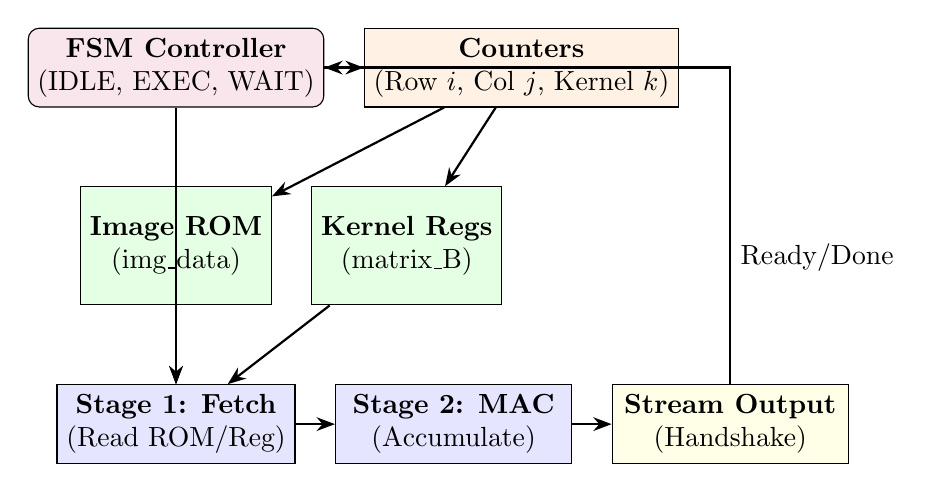
\begin{tikzpicture}[
    node distance=0.8cm and 0.5cm,
    process/.style={rectangle, draw=black, fill=orange!10, minimum width=3cm, minimum height=1cm, align=center},
    storage/.style={rectangle, draw=black, fill=green!10, minimum width=2cm, minimum height=1.5cm, align=center},
    ctrl/.style={rectangle, draw=black, fill=purple!10, minimum width=2.5cm, minimum height=1cm, rounded corners, align=center},
    arrow/.style={->, >=Stealth, thick}
]

% FSM
\node[ctrl] (fsm) {\textbf{FSM Controller}\\(IDLE, EXEC, WAIT)};

% Counters
\node[process, right=of fsm] (cnt) {\textbf{Counters}\\(Row $i$, Col $j$, Kernel $k$)};

% Datapath
\node[storage, below=1cm of fsm] (rom) {\textbf{Image ROM}\\(img\_data)};
\node[storage, right=0.5cm of rom] (kernel) {\textbf{Kernel Regs}\\(matrix\_B)};

% Pipeline
\node[process, below=1cm of rom, fill=blue!10] (fetch) {\textbf{Stage 1: Fetch}\\(Read ROM/Reg)};
\node[process, right=0.5cm of fetch, fill=blue!10] (mac) {\textbf{Stage 2: MAC}\\(Accumulate)};

% Output
\node[process, right=of mac, fill=yellow!10] (stream) {\textbf{Stream Output}\\(Handshake)};

% Connections
\draw[arrow] (fsm) -- (cnt);
\draw[arrow] (fsm) -- (fetch);
\draw[arrow] (cnt) -- (rom);
\draw[arrow] (cnt) -- (kernel);
\draw[arrow] (rom) -- (fetch);
\draw[arrow] (kernel) -- (fetch);
\draw[arrow] (fetch) -- (mac);
\draw[arrow] (mac) -- (stream);
\draw[arrow] (stream) |- (fsm) node[pos=0.2, right] {Ready/Done};

\end{tikzpicture}
\caption{卷积模块内部微架构示意图}
\end{figure}

\textbf{设计要点:}
\begin{itemize}
    \item \textbf{FSM}:控制计算流程,处理握手暂停。
    \item \textbf{流水线}:将计算拆分为取数(Fetch)和累加(MAC)两级,优化时序。
    \item \textbf{计数器}:$i, j$ 遍历图像像素,$k$ 遍历卷积核权重。
\end{itemize}

\newpage

\section{数据流控制方案}

系统采用“输出固定(Output Stationary)”的数据流模式,并结合反压机制(Backpressure)确保数据传输的可靠性。

\begin{figure}[H]
\centering
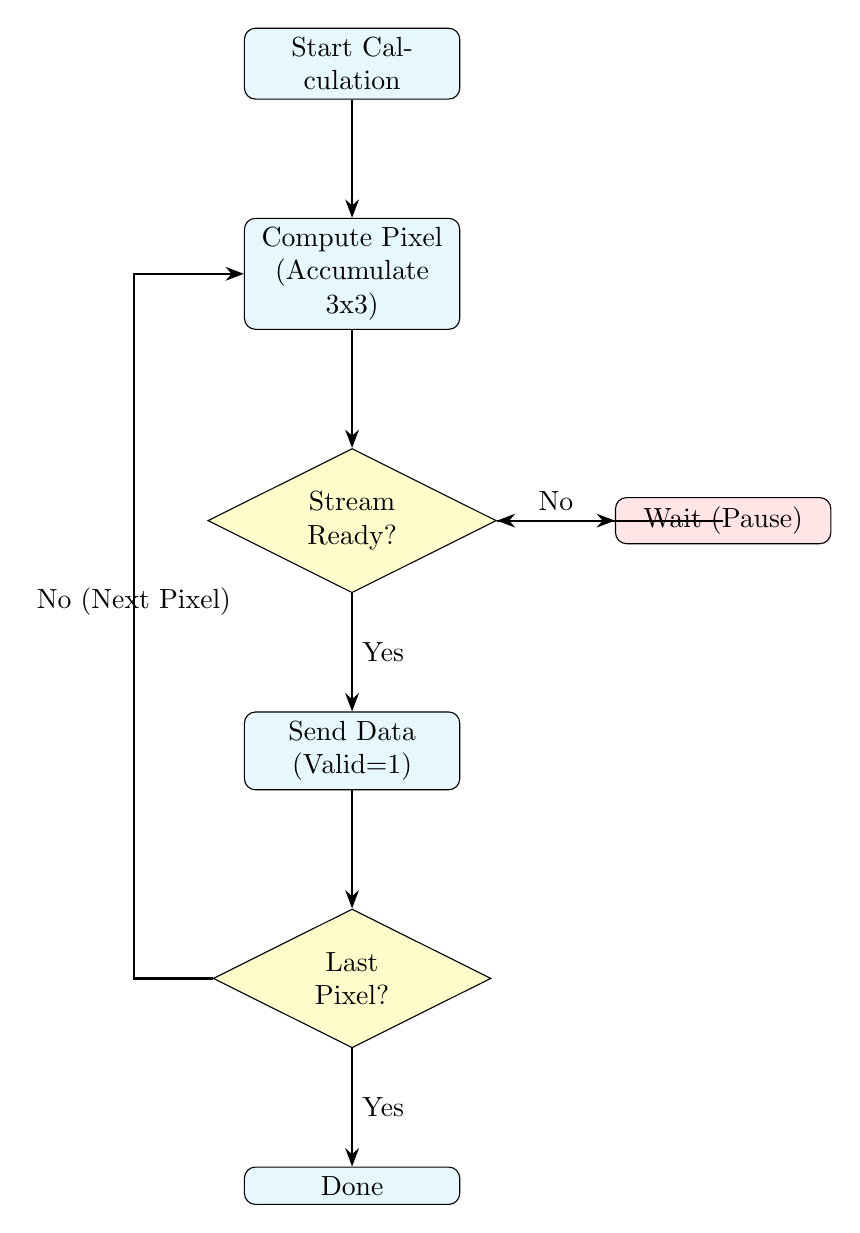
\begin{tikzpicture}[
    node distance=1.5cm,
    block/.style={rectangle, draw, fill=cyan!10, text width=2.5cm, align=center, rounded corners},
    decision/.style={diamond, draw, fill=yellow!20, text width=1.5cm, align=center, aspect=2},
    arrow/.style={->, >=Stealth, thick}
]

\node[block] (start) {Start Calculation};
\node[block, below=of start] (calc) {Compute Pixel\\(Accumulate 3x3)};
\node[decision, below=of calc] (check) {Stream\\Ready?};
\node[block, right=of check, fill=red!10] (wait) {Wait (Pause)};
\node[block, below=of check] (send) {Send Data\\(Valid=1)};
\node[decision, below=of send] (finish) {Last\\Pixel?};
\node[block, below=of finish] (done) {Done};

\draw[arrow] (start) -- (calc);
\draw[arrow] (calc) -- (check);
\draw[arrow] (check) -- node[right] {Yes} (send);
\draw[arrow] (check) -- node[above] {No} (wait);
\draw[arrow] (wait) |- (check);
\draw[arrow] (send) -- (finish);
\draw[arrow] (finish) -- node[right] {Yes} (done);
\draw[arrow] (finish.west) -- ++(-1,0) |- node[near start, above] {No (Next Pixel)} (calc);

\end{tikzpicture}
\caption{数据流与反压控制流程图}
\end{figure}

\textbf{控制策略:}
\begin{itemize}
    \item \textbf{计算流}:固定一个输出像素,累加完所有权重后才输出。
    \item \textbf{反压机制}:在输出前检查 \texttt{stream\_ready}。若下游忙(Ready=0),FSM 暂停在 \texttt{WAIT} 状态,保持数据有效但不发送,防止丢包。
\end{itemize}

\newpage

\section{性能优化策略}

主要采用了流水线(Pipelining)和资源复用策略来提升频率并减少资源消耗。

\begin{figure}[H]
\centering
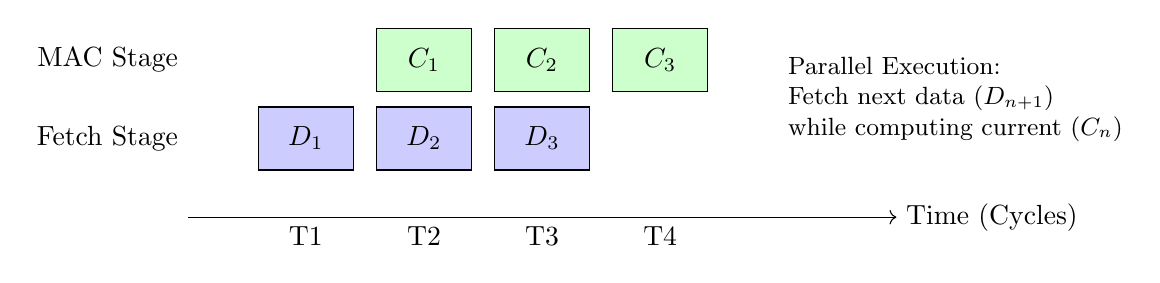
\begin{tikzpicture}[
    x=1.5cm, y=1cm,
    stage/.style={rectangle, draw, fill=white, minimum width=1.2cm, minimum height=0.8cm},
    arrow/.style={->, >=Stealth}
]

% Time axis
\draw[->] (0,0) -- (6,0) node[right] {Time (Cycles)};

% Pipeline Rows
\node[anchor=east] at (0, 1) {Fetch Stage};
\node[anchor=east] at (0, 2) {MAC Stage};

% Cycle 1
\node[stage, fill=blue!20] at (1, 1) {$D_1$};
\node[below] at (1,0) {T1};

% Cycle 2
\node[stage, fill=blue!20] at (2, 1) {$D_2$};
\node[stage, fill=green!20] at (2, 2) {$C_1$};
\node[below] at (2,0) {T2};

% Cycle 3
\node[stage, fill=blue!20] at (3, 1) {$D_3$};
\node[stage, fill=green!20] at (3, 2) {$C_2$};
\node[below] at (3,0) {T3};

% Cycle 4
\node[stage, fill=green!20] at (4, 2) {$C_3$};
\node[below] at (4,0) {T4};

% Annotation
\node[right, align=left, font=\small] at (5, 1.5) {Parallel Execution:\\Fetch next data ($D_{n+1}$)\\while computing current ($C_n$)};

\end{tikzpicture}
\caption{流水线优化示意图}
\end{figure}

\textbf{优化措施:}
\begin{itemize}
    \item \textbf{流水线设计}:将复杂的乘累加操作拆解。虽然单次计算延迟增加(Latency),但缩短了关键路径,提高了系统吞吐率(Throughput)。
    \item \textbf{资源复用}:卷积运算复用了矩阵乘法的 DSP 乘法器资源,避免了为卷积单独实例化大量乘法器,节省了 FPGA 面积。
\end{itemize}

\end{document}
